%%
%  ******************************************************************************
%  * #file    Szablon_raportu_EN_Latex.tex
%  * #author  Adrian Wójcik   adrian.wojcik(at)put.poznan.pl
%  *          
%  * #commit  Patryk Kościk   koscikpatryk(at)gmail.com
%  *          Modified the template for Projekt przejsciowy purposes          
%  *          
%  * #version 1.0
%  * #date    09-Mar-2022
%  * #brief   PROJPRZEJ
%  *
%  ******************************************************************************
%%  
\documentclass[11pt, a4paper]{article}

\usepackage{SM_template}

% Wypełnijcie te dyrektywy zgodnie z waszym tematem
% \lab      -> NAZWA CZUJNIKA, np.: 'DHT22'
% \comment  -> Króciutki opis co to, np.: 'Cyfrowy budżetowy czujnik temperatury'
%
\lab{Dioda LED RGB SMD}
\comment{Trójkolorowa dioda emitująca światło przeznaczona do montażu powierzchniowego}
\author{Antoni Borowski}

% Absolutny zakaz dotykania tego tutaj bo jak dotkiecie to coś jebnie
\university{Politechnika Poznańska}
\faculty{Wydział Automatyki, Robotyki i Elektrotechniki}
\institute{Instytut Robotyki i Inteligencji Maszynowej}
\department{Zakład Sterowania i Elektroniki Przemysłowej}
\addbibresource{bib/KY-009.bib}
\nocite{*}


%%
%
% Początek dokumentu
%
%%
\begin{document}

%% Strona tytułowa %%
\mainpage{{KY-009/dioda}}
\newpage

\section*{Opis elementu} \addcontentsline{toc}{section}{Wstęp}
Moduł KY-009 składa się z diody LED RGB (Red, Green, Blue) SMD (Surface Mount Technology) 5050 oraz czterech pinów męskich. Moduł należy podłączać poprzez rezystor, by zapobiec przepaleniu samej diody. 

\vspace{0.5cm}
\begin{figure}[h]
\centering
\begin{subfigure}{.5\textwidth}
  \centering
  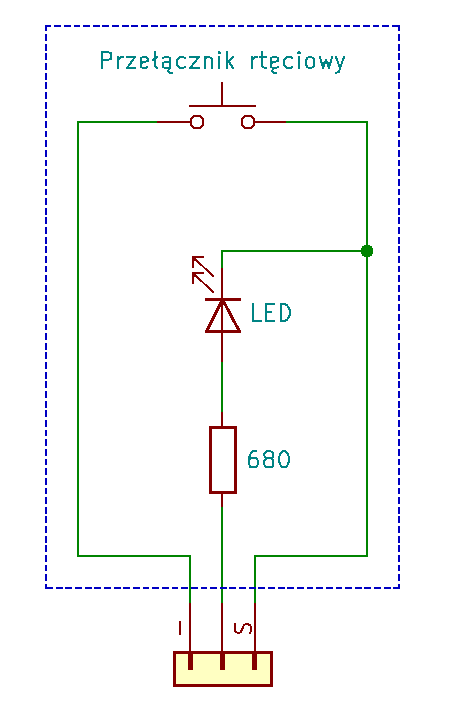
\includegraphics[width=.4\linewidth]{fig/KY-009/zdj_modułu/modul}
  \caption{Moduł KY-009 \cite{ArduinoModules:RGB}}
  \label{fig:sub1}
\end{subfigure}%
\begin{subfigure}{.5\textwidth}
  \centering
  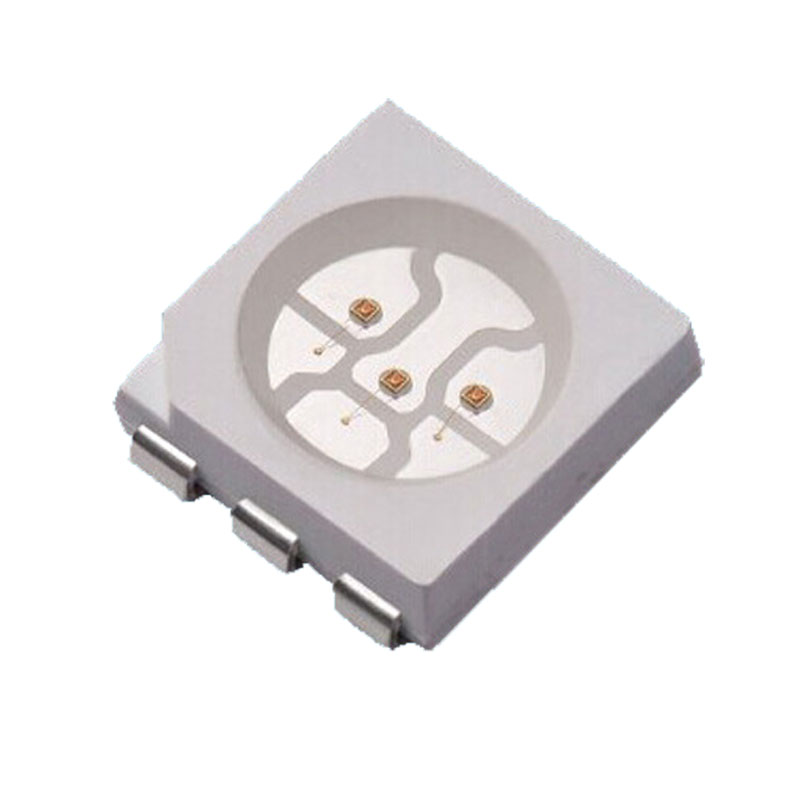
\includegraphics[width=.62\linewidth]{fig/KY-009/zdj_modułu/dioda2}
  \caption{Dioda LED RGB SMD \cite{LED:LED}}
  \label{fig:sub2}
\end{subfigure}
\caption{Zdjęcia poglądowe na czujnik i samą diodę}
\label{fig:test}
\end{figure}
\vspace{1cm}

LED (light emitting diode) jest elementem półprzewodnikowym, który wytwarza światło kiedy przepływa przez niego prąd od anody do katody. Dioda RGB to w zasadzie 3 LED w jednej obudowie, gdzie każda z nich wytwarza światło innego koloru (czerwone, zielone, niebieskie). W tym przypadku 3 diody mają wspólną katodę.
\vspace{0.5cm}
\begin{figure}[h]
\centering
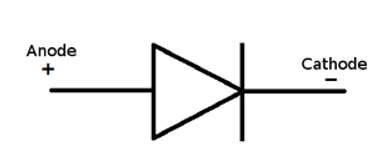
\includegraphics[width=.6\linewidth]{fig/KY-009/zasada_dzialania/LED symbol.png}
\caption{Schemat diody \cite{Wiki:Diode}}
\label{fig:sub2}

\end{figure}
\vspace{0.5cm}
\newpage
Dioda LED RGB SMD jest komponentem, który przeznaczony jest do montażu powierzchniowego na płytce z nadrukowanym obwodem. Cechą charakterystyczną komponentu jest jego niewielki rozmiar oraz kompatybilność ze złożonymi układami scalonymi. Dzięki powyższym zaletom, długiej żywotnośi oraz szerokiemy kątowi emisji światła, znajduje wiele zastosowań, m.in: w taśmach, modułach, oprawach, żarówkach, oświetlaczach i innych rodzajach źródeł światła.

\section*{Użycie czujnika}

Poniżej znajduje się tabela z połączeniami, schemat elektryczny oraz przykładowa konfiguracja GPIO dla modułu KY-009 

\subsection*{Połączenie fizyczne}

\vspace{0.5cm}
\begin{table}[h!]
    \centering
    \begin{tabular}{|c|c|c|c|} 
        \hline
        \multicolumn{2}{|c|}{NUCELO-F746ZG} & \multicolumn{2}{c|}{SENSOR}  \\ 
        \hline
        Etykieta & Port i numer pinu       & Nr pinu & Etykieta           \\ 
        \hline
        GND      & -                       & 1       & -              \\
        GPIO3    & PB7                     & 4       & -              \\
        GPIO1    & PB0                     & 2       & -              \\
        GPIO2    & PB14                     & 3       & -              \\
        \hline
    \end{tabular}
    \caption{Instrukcja połączeń}
\end{table}
\vspace{0.5cm}

\vspace{0.5cm}
\begin{figure}[h!]
    \centering
    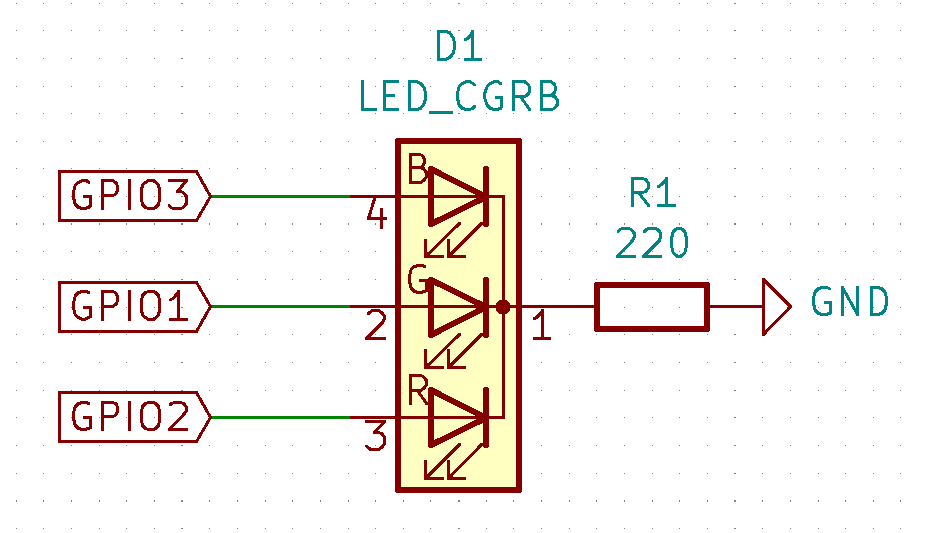
\includegraphics[width=12cm]{fig/KY-009/polaczenie_modulu/polaczenie.png}
    \caption{Połączenie elektryczne}
    \label{fig:my_label}
\end{figure}
\vspace{0.5cm}

\newpage

\subsection*{Kongiuracja IOC}

\vspace{0.5cm}
\begin{figure}[h!]
    \centering
    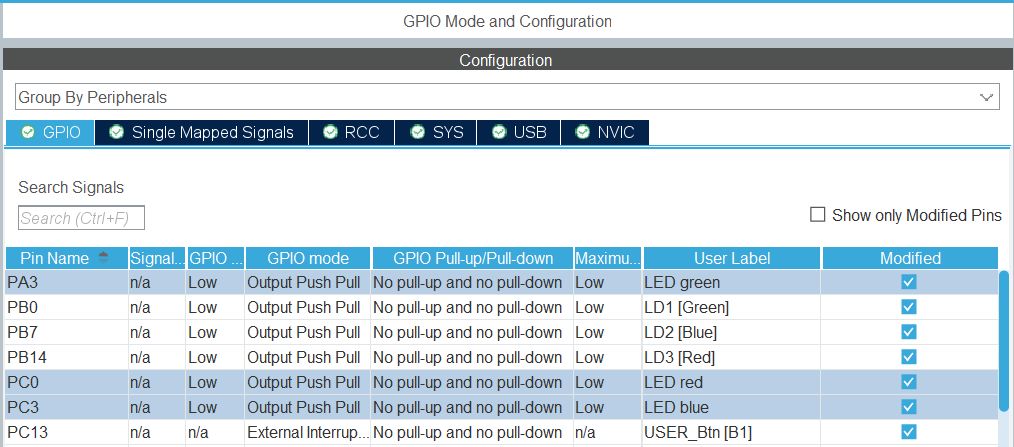
\includegraphics[width=16cm]{fig/KY-009/polaczenie_modulu/gpio1.png}
    \caption{Przykładowa konfiguracja GPIO mikrokotnrolera}
    \label{fig:my_label}
\end{figure}

\vspace{1cm}

\subsection*{Działanie}
Po podłączeniu modułu do mikroprocesora STM32 poprzez rezystor, dioda zaczyna świecić; przykładowy kod zawarty w suplemencie implementuje tryb świecenia polegający na zmianie koloru co sekundę - z zielonego na czerwony, z czerwonego na niebieski, z niebieskiego na zielony. 

\begin{figure}[h!]
    \centering
    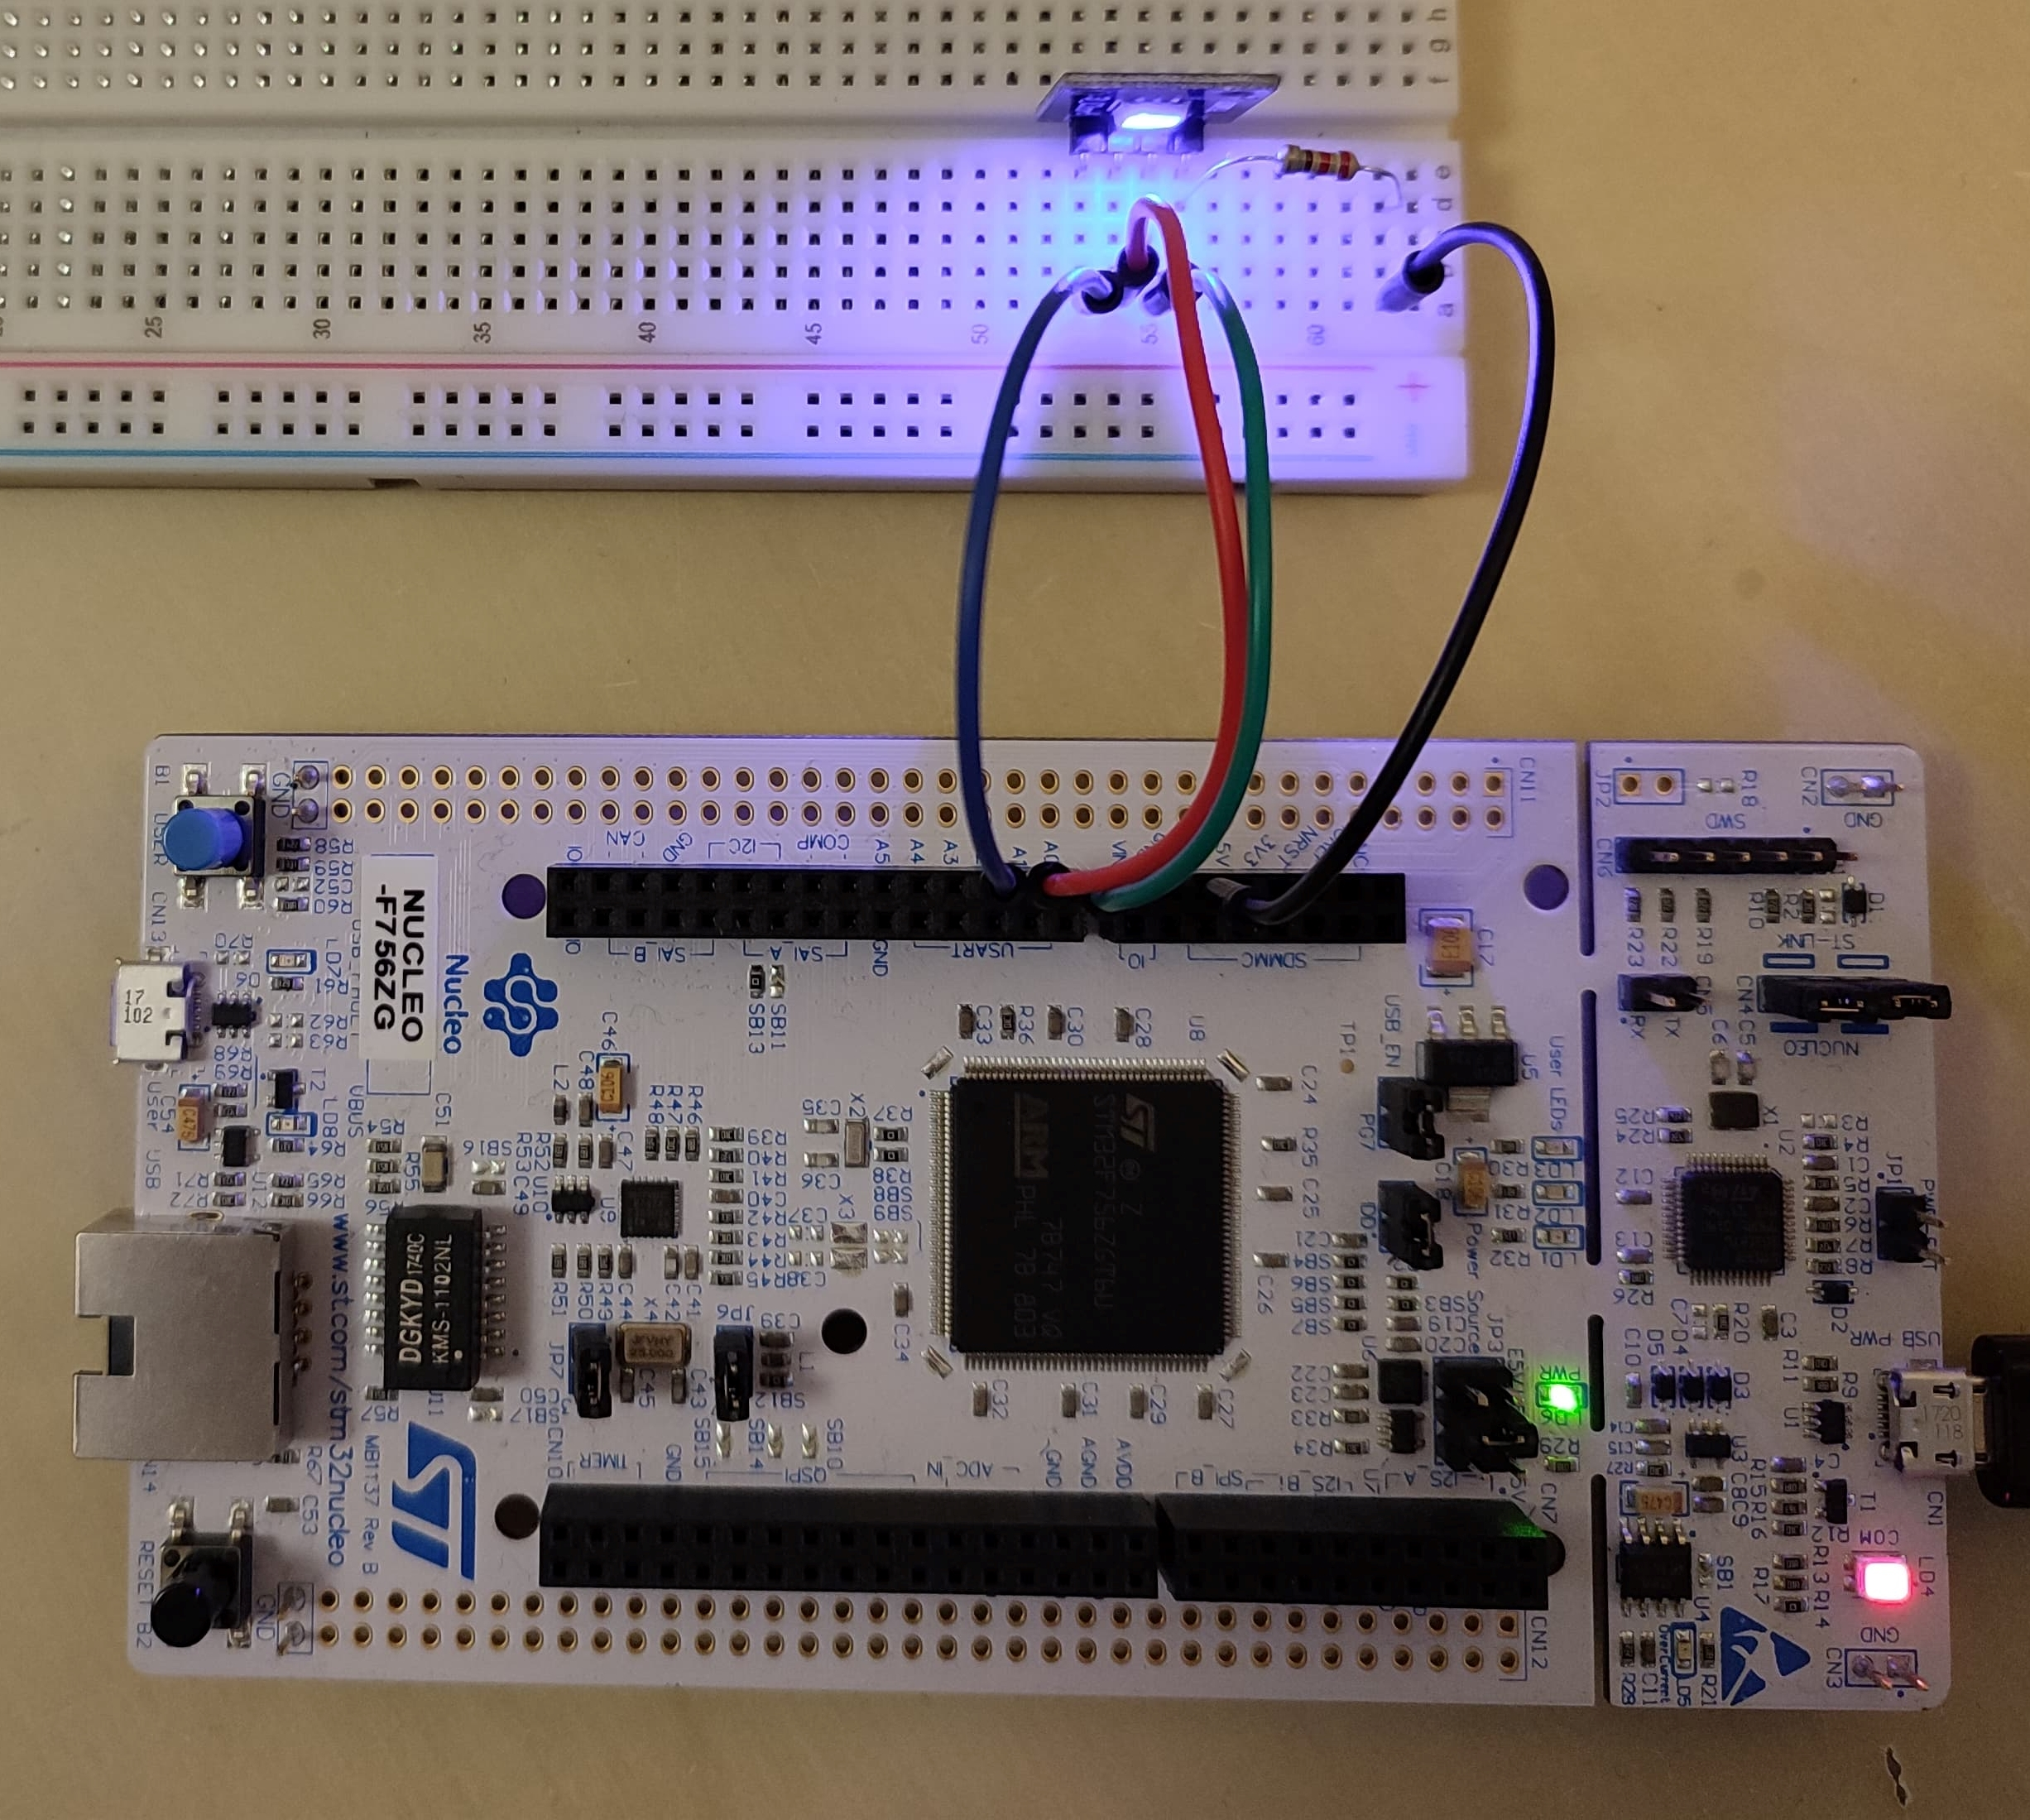
\includegraphics[width=8.8cm]{fig/KY-009/działanie_ukladu/dzialanie.jpg}
    \caption{Podłączony moduł i świecąca dioda}
    \label{fig:my_label}
\end{figure}

\newpage
Przykładowy kod programujący moduł KY-007 został zawarty w materiałach dodatkowych znajdujących się pod koniec rozdziału. Materiał obrazujący działanie układu znajduje się w suplemencie wideo.

\printbibliography[heading=bibintoc]

\end{document}